%% ceci est un commentaire 
%% il faut toujours commencer par \documentclass[type de papier, taille de texte]{sytle du document}
\documentclass[a4paper,10pt]{report} %%%% sytle du document : report/book/article


%%%%%%%%%%%%%%%%%%%%%%%%%%%%%%%%%%%%%%%%%%%%%%%%%%%%%%%%%%%%%%%%%%%%%%%%%%%%%%%
%% la suite est une collection des "package" ou des "librararies" pour utiliser des codes spécifiques
%% il vous suffit de les copie-coller quand vous créez un nouveau document TeX (ou bien en ajouter plus si besoin).
\usepackage[utf8]{inputenc} %% pour les accents en français
\usepackage[frenchb]{babel} %% pour un format français
\usepackage{graphicx} %% pour afficher des graphiques
\usepackage{amsmath} %% pour écrire des symboles (maths), des équations, etc.
\usepackage{amssymb}
\usepackage{color}
\usepackage{bm} %% pour lister des citations/la biblio
\usepackage{hyperref} %% pour inserer des liens internet
\usepackage{cleveref} %% pour faire des références uax équations, tableaux, etc.
%\usepackage{setspace} %% pour changer l'espace entre les lignes
%\linespread{1.6} %% pour changer l'espace entre les lignes












%%%%%%%%%%%%%%%%%%%%%%%%%%%%%%%%%%%%%%%%%%%%%%%%%%%%%%%%%%%%%%%%%%%%%%%%%%%%%%%
\title{\textbf{Etude d'un profil NACA avec Comsol}} %% choissez un titre approprié à votre sujet
\author{par\\ZHANG Xunjie\\pour le UE Atelier Numérique en Mécanique M1 } %% utilisez \\ pour une novuelle ligne
\date{fait le 29 mai 2017} %% pour afficher la date actuelle commenter cette ligne














%%%%%%%%%%%%%%%%%%%%%%%%%%%%%%%%%%%%%%%%%%%%%%%%%%%%%%%%%%%%%%%%%%%%%%%%%%%%%%%
%% TOUT ce qui va dans votre rapport doit être entre \begin{document} & \end{document}
\begin{document}
\selectlanguage{french} %% format français
\maketitle %% pour afficher le titre
\tableofcontents %% pour afficher/compiler le sommaire automatiquement
\listoffigures %% pour lister les figures
%%%%%%%%%%%%%%%%%%%%%%%%%%
%%%%%%%%%%%%%%%%%%%%%%%%%%%%%%%%%%%%%%%%%%%%%%%%%%%%%%%%%%%%%%%%%%%%%%%%%%%%%%%
\chapter{Introduction} 
\section{Introduction}
On se propose d’étudier un profil NACA avec COMSOL. On considère l’écoulement autour d’un profil NACA en incidence (angle $\alpha$). L'objectif de L’objectif de l’étude est de déterminer la force de portance et son point d’application(aussi appelé centre de poussée) pour différentes incidences$-10<{\alpha}<20$ à  l’aide du logiciel COMSOL, on effectuera d'abord une étude du profil NACA0012(un profil symétrique)en utilisant la modélisation potentielle vue en cours avec la condition de Kutta Joukovsky.Ensuite, on va étudier un profil NACA cambré à 4 chiffres qui est donnée par la nomenclature NACA.

\section{Problèm physique}

\begin{figure}[h]
\centering
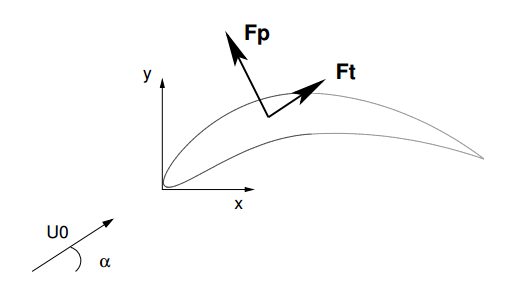
\includegraphics[width=0.9\textwidth]{fig/figure1.png}
\caption{Problem physique etude}
\end{figure}

\chapter{Modélisation du problème } 
\section{Theorique pour NACA symétrique}%% pour commencer une section
On fait plusieurs hypothèses pour simplifier notre problème :
\begin{enumerate} 
	\item L'écoulement est stationnaire
	\item Le fluide est incompressible
	\item Le fluide est parfait (on pourra donc prédire la portance mais pas la force de traînée car on néglige les effets des forces de viscosité)
    \item L'écoulement est bi-dimensionnel (théorie de l'aile d'envergure infinie)
    
\end{enumerate} 
le modèle suivant pour $\vec{U}=\left\{
\begin{aligned}
u&= \frac{\partial{\psi}}{\partial{y}} \\
v&= -\frac{\partial{\psi}}{\partial{x}} \\
\end{aligned}
\right.
$
En faisant le bilan de masse et le bilan de quantité de mouvement, on obtient:
$$\left\{
\begin{aligned}
div\vec{U}&=0=&\frac{\partial{u}}{\partial{x}}+\frac{\partial{v}}{\partial{y}} \\
rot\vec{U}&=0=&\frac{\partial{v}}{\partial{x}}-\frac{\partial{u}}{\partial{y}} \\
\end{aligned}
\right.
$$
Et On va donc utiliser la fonction de courant  , et on s'intéressera aux lignes de courant ($\psi = cste$) qui sont tangentes en chaque point au vecteur vitesse.
$$\left\{
\begin{aligned}
div\vec{U}&=div(\vec{grad}\psi)=\Delta\psi=0 \\
rot\vec{U}&=rot(\vec{grad}\psi)=0 \\
\end{aligned}
\right.
$$
On met un écoulement qui arrive avec
une vitesse $U_{0}$,et l'angle inclinée de la $\alpha$ donc $u=U_{0}sin(\alpha)$,$v=U_{0}cos(\alpha)$
Et $ \Delta\psi=0 $ :
$$\left\{
\begin{aligned}\frac{\partial{\psi}}{\partial{y}}=U_{0}cos(\alpha)  \\
\frac{\partial{\psi}}{\partial{x}}=-U_{0}sin(\alpha)  \\
\end{aligned}
\right.
$$
Alors on a $$\psi_{\infty}=U_{0}(cos(\alpha) y-sin(\alpha)x)$$
On s'intéresse aux points d'arrêt.La vitesse est nulle en ces points et il y a une surpression.Au niveau du bord de fuite, la ligne de courant est tangente au bord car le profil est mince. La valeur de $\psi$ sur $\Gamma_{1}$doit être fixée telle que l'on n'ait pas de contournement autour du bord de fuite, c'est la condition de Kutta-Joukovski. Cela va déterminer la valeur de la circulation autour du profil.
Donc, on décomposé en deux problèmes pour générer une circulation de vitesse.On a donc le problème sous la forme:$\psi=\psi_{1}+\beta\psi_{2}$ :

$$\left\|
\begin{aligned}
Problem 1\\
\Delta\psi_{1}=0 \\
\psi_{1}=U_{0}y &&sur\Gamma_{0} \\
\psi_{1}=0 &&sur\Gamma_{1}\\
\end{aligned}
\right.
$$
$$\left\|
\begin{aligned}
Problem 2\\
\Delta\psi_{2}=0 \\
\psi_{2}=0 &&sur\Gamma_{0} \\
\psi_{2}=1 &&sur\Gamma_{1}\\
\end{aligned}
\right.
$$
Sur le point d'arrêt,on a un angle de tangente sur le bord de fuite $\theta$ et $\nabla\vec{\psi}*\vec{U}=0$. Dans le cas symétrique, $\theta=0$. Donc:$$\frac{\partial{\psi}}{\partial{x}}{\Big|_{\beta}}=0 $$
Avec $$\beta=\frac{-\frac{\partial{\psi_{1}}}{\partial{x}}}{\frac{\partial{\psi_{2}}}{\partial{x}}}$$


%%%%%%%%%%%%%%%%%%%%%%%%%%%%%%%%%%%%%%%%%%%%%%%%%%%%%%%%%%%%%%%%%%%%%%%%%%%%%%%
\section{Étude du profil NACA cambré}
On utilise python pour obtenir notre NACA cambré , et on a la profile ici avec la ligne moyenne :

\begin{figure}[h]
\centering
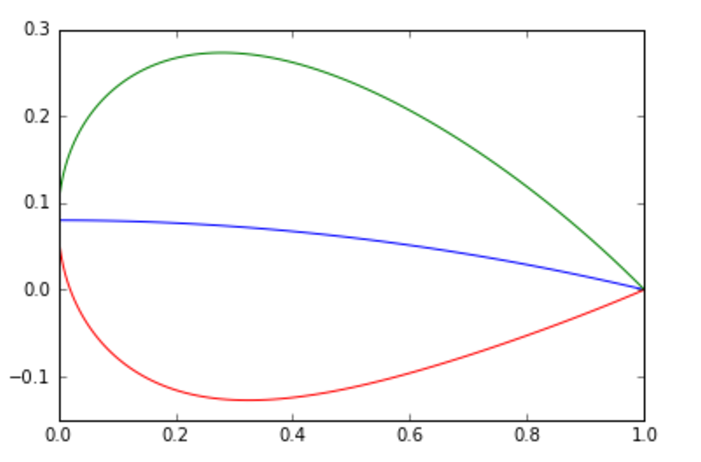
\includegraphics[width=0.7\textwidth]{fig/figure2.png}
\caption{	Profile de NACA cambré}
\end{figure}


On fait la même étude pour le profil cambre NACA.Pour obtenir la géométrie du profil, on écrit un fichier en format.dxf par Python. Pour cette étude, il faut recalculer la nouvelle  tangente au bord de fuite, car il n'est plus horizontale. Pour trouver le $\theta$,on choisit un point en $x=1.1$, alors on peut obtenir l'angle $\theta=-0.074$ sur la programme de python. On a $\psi=\psi_{1}+\beta\psi_{2}$,  $\nabla\vec{\psi}*\vec{U}=0$. Donc:
$$\left\{
\begin{aligned}
\frac{\partial{\psi}}{\partial{x}}{\Big|_{\beta}}*cos(\theta)=0 \\
\frac{\partial{\psi}}{\partial{y}}{\Big|_{\beta}}*sin(\theta)=0 \\
\end{aligned}
\right.
$$
Avec $$\beta=\frac{-\frac{\partial{\psi_{1}}}{\partial{x}}\cos(\theta)+\frac{\partial{\psi_{1}}}{\partial{y}}\sin(\theta)}{\frac{\partial{\psi_{2}}}{\partial{x}}\cos(\theta)-\frac{\partial{\psi_{2}}}{\partial{y}}\sin(\theta)}$$
\section{Résultal pour NACA cambré}
On fait ensuite une étude paramétrique avec $-10<\alpha<20$.
\subsection{Isovaleur Potentiel}
\begin{figure}[h]
\centering
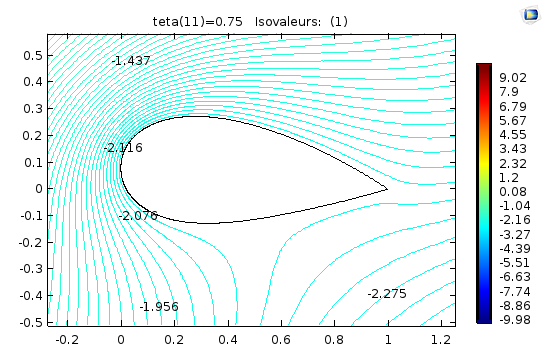
\includegraphics[width=1.0\textwidth]{fig/figure3.png}
\caption{	Isovaleur Potentiel d'un profile de NACA cambré}
\end{figure}

Comme dans la figure 2.2 , on plot la figure de isolvaleur de potentiel . Dans la extrémité du profile , la ligne est bien s'installé . On dit que on trouve une bonne profile d'isovaleur de potentiel .

\subsection{Pression d'une profile d'un $\alpha$}
Dans la figure 2.3 ,  on a les couleurs rouge vers lue qui sont négatives . Cette figure est trouvées pour le premiere $\alpha$ . On remarque dans l'extremité a gauche , on trouve la pression maximal negative .
\begin{figure}[h]
\centering
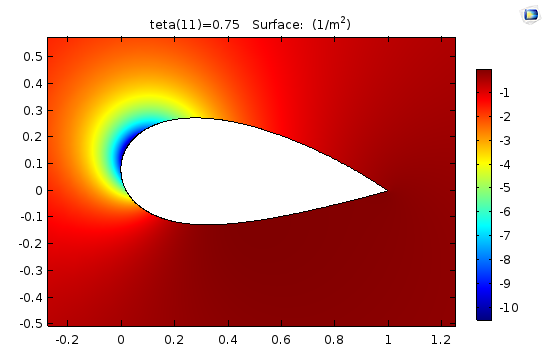
\includegraphics[width=1.0\textwidth]{fig/figure4.png}
\caption{Pression d'un profile d'un $\alpha$ NACA cambré}
\end{figure}


\subsection{Potentiel de sonde des $\alpha$}

\begin{figure}[h]
\centering
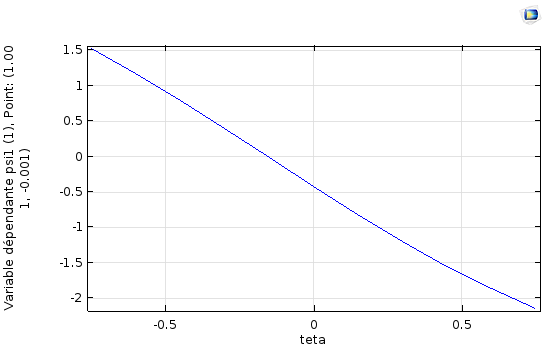
\includegraphics[width=1.0\textwidth]{fig/figure5.png}
\caption{	Potentiel de sonde des $\alpha$ d'un profile de NACA cambré}
\end{figure}

Dans la figure 2.4 , on plot la potentiel de sonde . Cette sonde est une pointe qui se trouve dans le ligne moyenne d'un profile . Dans Python on met coordonée x est 1.001 , et trouve coordonnée y est -0.001 . Dans ce cas , $\alpha$va évaluer -0.75 à 0.75 . Cette fonction est presque une ligne droite . Elle est bien satisfait la solution analytoque .
\subsection{Portance pour tous les $\alpha$}
\begin{figure}[h]
\centering
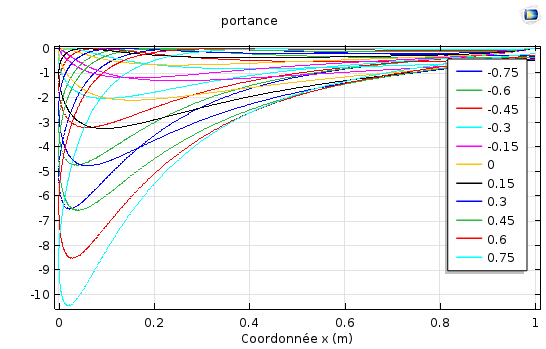
\includegraphics[width=1.0\textwidth]{fig/figure6.png}
\caption{	Portance pour tous les $\alpha$ d'un profile de NACA cambré}
\end{figure}

Dans la figure 2.5 , on plot les portrances pour tous les $\alpha$ . Pour une valeur de $\alpha$ , la surface entre la ligne haut et la ligne bas est la force de portance . Comme on voir dans la figure 2.5 , quand $\alpha$ est 0.75 , la force de portance est maximal .


\chapter{Trouvez le centre de portance avce PYTHON} 
\section{Étude laminaire ,couche limite}
\begin{figure}[h]
\centering
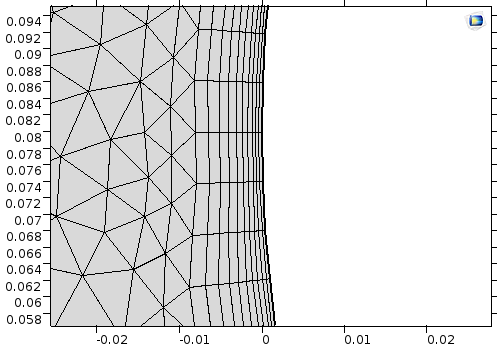
\includegraphics[width=0.9\textwidth]{fig/figure8.png}
\caption{	Portance pour tous les $\alpha$ d'un profile de NACA cambré}
\end{figure}
Dans la figure 3.1 , on etude la couche limite , dans comsol proche de la naca cambré , on fait plus de maillages rectange pour bien développer la couche limite .

Dans la figure 3.2 ,on lance comsol et etude cette profil avce les maillages on defini par utilisateur , et on trouve la profil de vitess .

Dans la figure 3.3 on bien trouve  la force portance d'après etude de couche limite .



\begin{figure}[h]
\centering
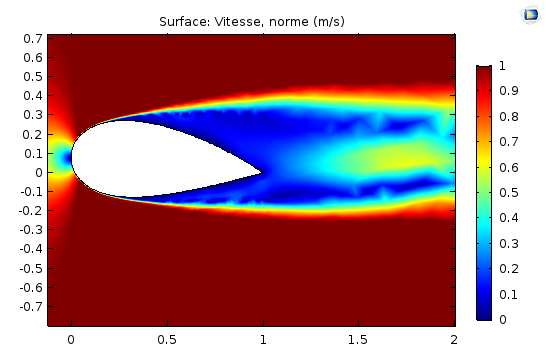
\includegraphics[width=0.8\textwidth]{fig/figure9.png}
\caption{	Portance pour tous les $\alpha$ d'un profile de NACA cambré}
\end{figure}


\begin{figure}[h]
\centering
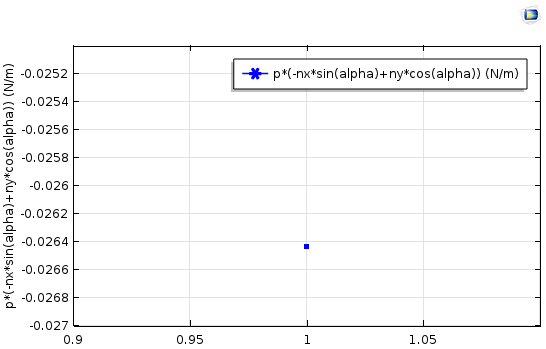
\includegraphics[width=0.7\textwidth]{fig/figure10.png}
\caption{	Portance pour tous les $\alpha$ d'un profile de NACA cambré}
\end{figure}







\section{Le centre de poussée}
Le point d’application $P(x_{P},y_{P})$ (aussi appelé centre de poussée) de la résultante
des forces aérodynamiques $\vec{F}=\vec{F_{P}}+\vec{F_{t}}$ doit vérifier la relation suivante sur le moment de la résultante par rapport à un point $O$ quelconque:

$$\vec{OP}\land\vec{F}=\int_{s}\vec{OM}\land\vec{dF} $$
Avec $\vec{F}=\int_{s}-p\vec{n}dS$, $\vec{dF}=-p\vec{n}dS$,$M(x_{M},y_{M})$ un point du profil et $\vec{n}$ le vecteur normal sortant.
On a aussi $\vec{F}=\vec{F_{x}}\vec{x}+\vec{F_{y}\vec{y}}$. On peut ensuite calculer la position du centre de poussée en écrivant les relations sur le moment de chacune de ces forces projetées : 
$$\left\{
\begin{aligned}
x_{P}F_{y}=\int_{s}x_{M}dF_{y} \\
y_{P}F_{x}=\int_{s}y_{M}dF_{x}\\
\end{aligned}
\right.
$$


\begin{figure}[h]
\centering
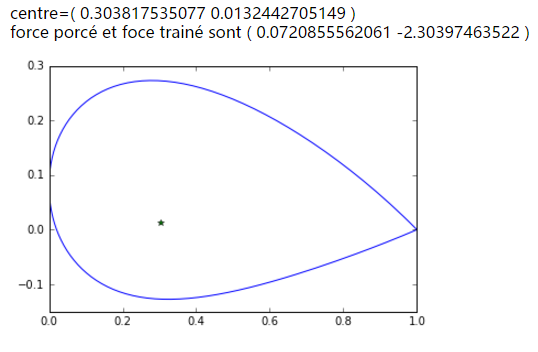
\includegraphics[width=1.0\textwidth]{fig/figure7.png}
\caption{	Centre de portace et les forces}
\end{figure}


\chapter{Conclusion} 
Dans cette séance de TP , on a fait une bonne modélisation d'un profil d'aile. Au début on utilise Python pour rediger notre profile NAVA cambré ,avec cette NACA cambré , on import sur Comsol, ensuite on utilise COMSOL pour etudier cette profile NACA cambré , on utilise la simulation pour trouver les pression , les isovaleurs de potentiel , ansi que les force portances . D'après Comsol , on obtient trois dossier 'coordonnées x , y , et pression . Avec ces trois dossiers , on reutilise python pour retrouver la profile NACA cambré , et trouver le centre de portance . On  a aussi la force pousé et la force trainée .
\\
\\ 

D'après cette etude de profile NACA , on connait , dans la vie quotidien , comment calculer les forces de pousées pour un aile avec une petite angle d'entrée . Et en d'autre paitie , on est plus similaire avec Python et Comsol , c'est très utile pour l'etude et travail. 



\end{document}
\grid
